\section{The Model}
This section will showcase the model made to express the design from \myref{cha:Design}.
For simplicity the introduction of the model in this chapter has split the model into two parts, an initializing phase and the main loop.
The complete model can be seen in \myref{app:UPPAAL} along with the code for the global and local declarations, including the functions used throughout the model.

The first part to be shown will be the initialization, which can be seen on \myref{fig:UPPAAL_Intitialization}

\begin{figure}
  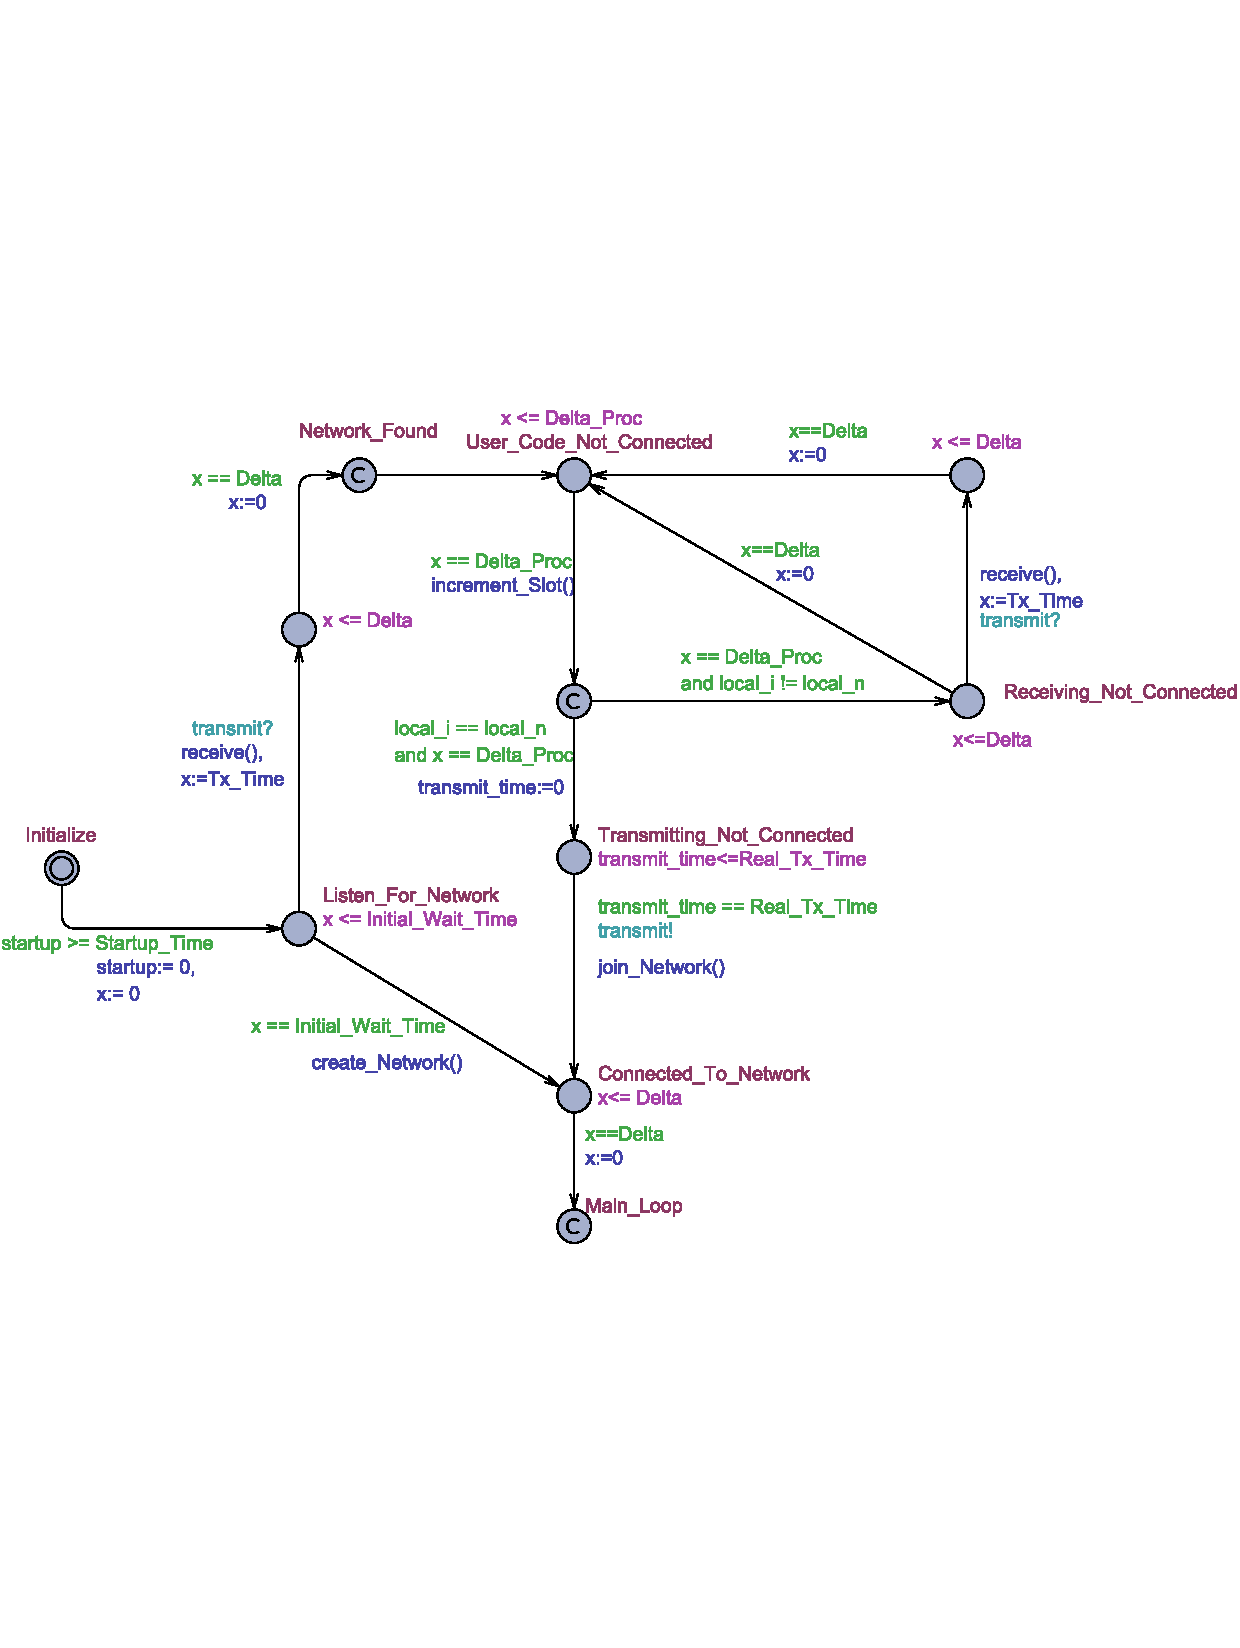
\includegraphics[width=1\textwidth]{Figures/Model/Device_Connecting.pdf} 
\caption{UPPAAL Model showing how the devices initialize.}
\label{fig:UPPAAL_Intitialization}
\end{figure}

The initial state has a clock \texttt{startup}, which makes sure that only one of the devices will be leaving the initial state at the same time.
When one of the devices leave this state, \texttt{startup} will reset, and another will leave the state when the \texttt{startup} once again reaches the desired time.
It has to be mentioned that this \texttt{Startup\_Time} has to be increased as the number of devices in the system increases.
This is because when the frame of the network becomes larger, \texttt{Startup\_Time} has to be increased to make sure that only one device has been released at a time for when en empty time-slot occurs.

With the current values in the model creating a network with six devices is doable.
While the other devices are waiting to be released, the device which was the first to leave will listen for a network, as there is obviously no network yet the device will fire the edge towards the \texttt{Creating\_Network} state.
The device will setup the initial values for the network, change its boolean \texttt{Connected} to true, and start the main loop.
When the next device leaves the initial stage, it will when it is listening for a network be successful as a network has just been created, which means that the device will move towards the committed state \texttt{Network\_Found} and reset the clock \texttt{x} to zero.
This state is committed as its purpose is simply context switching between receiving and performing user code.
When it has just received a transmission, the device which just transmitted will according to \myref{cha:Design} be performing user code, and so should the device trying to connect.

When \texttt{x} is equal to \texttt{Delta\_Com}, which is the time given to a device to perform user code, the device will change to the state \texttt{Network\_Found} once again.
In this state when \texttt{x} is not zero, the device checks whether \texttt{i}, which is the current time-slot, is the empty-time slot, if it is the device will transmit, and ultimately connect to the network, increasing the number of time-slots in the network according to the specifications from \myref{cha:Design}.
If the empty slot was not the current time-slot, the device will instead go to the state \texttt{Receiving\_Not\_Connected} where it will receive the other devices' transmissions, and once again reset \texttt{x} to zero, and perform user code, until eventually the empty-slot occurs, where it will connect to the network.

The committed state \texttt{Connected\_To\_Network} has 3 edge leaving it, one for receiving, one for transmitting, and one of executing user code.
The model can be seen on \myref{fig:UPPAAL_Connected}.

\begin{figure}
  
\includegraphics[width=1\textwidth]{Figures/Model/Device_Connected.pdf} 
\caption{UPPAAL Model showing the devices' main loop.}
\label{fig:UPPAAL_Connected}
\end{figure}

It works the roughly the same as the state \texttt{Network\_Found}, except the guard checking whether it is the empty time-slot instead checks whether it is the device's time-slot.
Another change is when the device is in the state \texttt{Receiving}, if nothing has been transmitted and the clock \texttt{x} is equal to \texttt{Delta} the device will go increment its \texttt{i\_local} value and go perform user code. 
This case happens whenever the empty slot is the current time-slot and no new device is trying to connect to the network.
For a specification of all the functions being used in this model, please have a look in \myref{app:UPPAAL}.

\section{Verifying the Model}

As mentioned in \myref{subsec:uppaal} it is possible to make queries to verify that some given properties are true.
\myref{sec:Pseudo} contains statements which should be true for a correctly connected network.
These statements can be written as queries in UPPAAL, which the tool will then determine to be correct or not. 
The queries in UPPAAL can be seen on \myref{lst:UPPAAL_Queries}.

\begin{lstlisting}[language={[GUI]Uppaal}, % use GUI flavor
columns={[l]flexible},
frameround=fftt, frame=shadowbox, rulesepcolor=\color{gray},label=lst:UPPAAL_Queries,
caption={Queries for the UPPAAL Model}]
1. A<> forall(i: id_t) Device(i).Connected
2. A[] not deadlock
3. A[] forall(i : id_t) forall(j : id_t)  Device(i).Transmitting and 
		Device(j).Transmitting imply i == j
4. A<> forall(i : id_t) forall(j : id_t) (Device(i).User_Code and 
		Device(j).User_Code and Device(i).local_i == Device(j).local_i)
5. A<> forall(i : id_t) forall(j : id_t) Device(i).local_n == Device(j).local_n
6. A<> forall(i : id_t) forall(j :id_t) Device(i).k != Device(j).local_n
7. A<> forall(i : id_t) forall(j : id_t) Device(i).k == Device(j).k imply i == j
8. A<> n == N+1
9. A<> forall(i : id_t)  Device(i).k < n and Device(i).k > 0
\end{lstlisting}

All of these queries will yield a true result when run with 6 devices on the model which has been shown.
More queries have been added to verify the model, an example is query 2.
A brief explanation of each query will be given below. 

\begin{description}
	\item [Query 1.] asks if for all possible state transitions, will it at some point be true that all devices in the system will be connected.
	\item [Query 2.] asks if there are no deadlocks in the model.
	\item [Query 3.] determines whether two different devices can be in the state \texttt{transmitting} at the same time.
	\item [Query 4.] will decide whether the devices local number of i, is the same when they are all in the state \texttt{User\_Code}.
	\item [Query 5.] asks if all devices has the same value of n in the local variable n.
	\item [Query 6.] asks if it false that any device has taken the empty time-slot as their own time-slot.
	\item [Query 7.] asks if any two devices have taken the same time-slot k.
	\item [Query 8.] asks if at some point is it always true that the number of time slots in the network is one larger than the number of devices in the system.
	\item [Query 9.] asks if all the time-slots in the network are less than n and larger than 0.
\end{description}

The queries 7-9 together make up the statement (e) from \myref{subsec:uppaal}, since if no devices have the same time-slot k and if the number of devices is one less than the number of time-slots and all time-slots are in the range [1,n-1] all number in this range must be a time-slot in the network.

Since all of these statements hold true, it is concluded that the model does indeed do what it was designed to do, and an implementation according to the specification should theoretically work and be possible to create.
